\chapter{トレースログ可視化ツール TraceLogVisualizer の実装}

\section{TraceLogVisualizerの全体像}

TLVの主機能は,2つの主たるプロセスと6種の外部ファイルによって実現される.
図\ref{fig:tlv}にTLVの全体像を示す.

2つの主たるプロセスとは,標準形式への変換と,図形データの生成である.
標準形式への変換は,任意の形式をもつトレースログを標準形式トレースログに変換する処理である.
この処理には外部ファイルとして変換元のトレースログファイル,リソースを定義したリソースファイル,リソースタイプを定義したリソースヘッダファイル,標準形式トレースログへの変換ルールを定義した変換ルールファイルが読み込まれる.

また,図形データの生成は,変換した標準形式トレースログに対して可視化ルールを適用し図形データを生成する処理である.
この処理には外部ファイルとして可視化ルールファイルが読み込まれる.
可視化ルールファイルとは図形と可視化ルールの定義を記述したファイルである.

TLVは,トレースログとリソースファイルを読み込み,ターゲットに対応したリソースヘッダファイル,変換ルールファイルの定義に従い,標準形式トレースログを生成する.
生成された標準形式トレースログに可視化ルールファイルで定義される可視化ルールを適用し図形データを生成した後,画面に表示する.


生成された標準形式トレースログと図形データは,TLVデータとしてまとめられ可視化表示の元データとして用いられる.
TLVデータはTLVファイルとして外部ファイルに保存することが可能であり,TLVファイルを読み込むことで,標準形式変換と図形データ生成の処理を行わなくても可視化表示できるようになる.

\begin{figure}[h]
\begin{center}
\includegraphics[scale=0.5]{img/tlv.eps}
\caption{TLVの全体像}
\label{fig:tlv}
\end{center}
\end{figure}

\subsection{Json}

リソースファイル,リソースヘッダファイル,変換ルールファイル,可視化ルールファイルは,Json(JavaScript Object Notation)\cite{Json}と呼ばれるデータ記述言語を用いて記述する.

Jsonは,主にウェブブラウザなどで使用されるECMA-262,revision 3準拠のJavaScript(ECMAScript)と呼ばれるスクリプト言語のオブジェクト表記法をベースとしており,RFC 4627としてで仕様が規定されている.
JsonはUnicodeのテキストデータで構成され,バイナリデータを扱うことは出来ない.
また,Jsonではシンタックスのみの規定がなされ,セマンティクスは規定されていない.

Jsonの特徴はシンタックスが単純であることである.
これは,人間にとっても読み書きし易く,コンピュータにとってもパースし易いことを意味する.
また,複数のプログラミング言語でJsonファイルを扱うライブラリが実装されており,異なる言語間のデータ受け渡しに最適である.
Jsonが利用可能なプログラミング言語としては,ActionScript, C, C++, C\#, ColdFusion, Common Lisp, Curl, D言語, Delphi, E, Erlang, Haskell, Java, JavaScript (ECMAScript), Lisp, Lua, ML, Objective CAML, Perl, PHP, Python, Rebol, Ruby, Scala, Squeakなどがある.

TLVの各ファイルのフォーマットにJsonを採用した理由はこれらの特徴による.
シンタックスが単純であることにより,ユーザの記述コスト,習得コストを低減させることができ,また,複数のプログラミング言語でパース可能であることによりファイルに可搬性を持たせることが出来るからである.

Jsonで表現するデータ型は以下のとおりであり,これらを組み合わせることでデータを記述する.
\begin{itemize}
\setlength{\itemsep}{0.5\itemsep}
\item 数値(整数,浮動小数点)
\item 文字列(Unicode)
\item 真偽値(true,false)
\item 配列(順序付きリスト)
\item オブジェクト(ディクショナリ,ハッシュテーブル)
\item null
\end{itemize}

Jsonの文法をEBNFと正規表現を用いて説明する.

Jsonはオブジェクトか配列で構成される.

\begin{EBNF}
JsonText = Object | Array;
\end{EBNF}

オブジェクトは複数のメンバをカンマで区切り,中括弧で囲んで表現する.
メンバは名前と値で構成され,名前のあとにはセミコロンが付く.
メンバの名前は文字列である.

\begin{EBNF}
Object = "{",Member,[{",",Member}],"}";
Member = String,":",Value;
\end{EBNF}

配列は複数の値をコンマで区切り,角括弧で囲んで表現する.

\begin{EBNF}
Array = "[",Value,[{",",Value}],"]";
\end{EBNF}

値は文字列,数値,オブジェクト,配列,真偽値,nullのいずれかである.
文字列はダブルクオーテーションで囲まれたUnicode列である.
数値は10進法表記であり,指数表記も可能である.

\begin{EBNF}
Value = String|Number|Object|Array|Boolean|"null";
String = /"([^"\]|\n|\"|\\|\b|\f|\r|\t|\u[0-9a-fA-F]{4})*"/;
Boolean = "true"|"false";
Number = ["-"],("0"|Digit1-9,[Digit]),[".",Digit],Exp;
Exp = ["e",[("+"|"-")],Digit];
Digit = /[0-9]+/;
Digit1-9 = /[1-9]/;
\end{EBNF}

以下にオブジェクトの例を示す.

\begin{File}
{
  "Image":{
    "Width":  800,
    "Height": 600,
    "Title":  "View from 15th Floor",
    "Thumbnail":{
      "Url":    "http://www.example.com/image/481989943",
      "Height": 125,
      "Width":  "100"
    },
    "IDs": [116, 943, 234, 38793]
  }
}
\end{File}

以下に配列の例を示す.

\begin{File}
[
  {
    "City":      "SAN FRANCISCO",
    "State":     "CA",
    "Zip":       "94107",
    "Country":   "US"
  },
  {
    "City":      "SUNNYVALE",
    "State":     "CA",
    "Zip":       "94085",
    "Country":   "US"
  },
  {
    "City":      "HEMET",
    "State":     "CA",
    "Zip":       "92544",
    "Country":   "US"
  }
]
\end{File}

\section{標準形式への変換}

標準形式トレースログへの変換は,トレースログファイルを先頭から行単位で読み込み,変換ルールファイルで定義される置換ルールに従い標準形式トレースログに置換していくことで行われる.変換ルールファイルの詳細は\ref{subsec:cnvFile}小節で説明する.

1つの置換ルールに対して複数の標準形式トレースログを出力可能である.
また,所望の標準形式トレースログに変換する際,トレースログファイルの情報だけでは足りない場合がある.
例として,TOPPERS/ASPカーネルというRTOSのトレースログを標準形式トレースログに変換することを考えてみる.
TOPPERS/ASPカーネルのトレースログを次に示す.

\begin{File}
[1000]task 1 becomes RUNNABLE
[1005]dispatch to task 1.
[1100]task 1 becomes WAITING
\end{File}

上記のトレースログの内容を簡単に説明すると,時刻1000にタスクIDが1のタスクの状態がRUNNABLEになり,時刻1005に同タスクがディスパッチされ,時刻1100に同タスクの状態がWAITINGになったことを示している.
この場合,標準形式トレースログは次のように出力されることが要求される.
なお,説明のため簡略化しており,実際の変換結果とは異なる.

\begin{File}
[1000]Task(id==1).activate()
[1000]Task(id==1).state = RUNNABLE
[1005]Task(state==RUNNING).state=RUNNABLE
[1005]Task(id==1).state = RUNNING
[1100]Task(id==1).state = WAITING
\end{File}

元のトレースログが3行なのに対し,要求される標準形式トレースログは5行となっている.
これは,標準形式トレースログの1行目と3行目が状況により追加される必要があるからである.
標準形式トレースログの1行目は,元のトレースログの1行目に対応しており,起動(\verb|activate()|)というタスクの振る舞いを可視化したいという要求があるため追加される必要がある.
また,標準形式トレースログの3行目は,元のトレースログの2行目に対応しており,すでに起動しているタスクがプリエンプトされて状態がRUNNABLEになるという情報が元のトレースログに存在しないため追加される必要がある.
しかしながら,これら標準形式トレースログの追加が必要になるのは一定の条件下のみである.
標準形式トレースログの1行目は,タスクIDが1のタスクの状態が,時刻1000未満のときにDORMANTである場合だけである.
これは,起動という状態遷移を行うのが状態がDORMANTからRUNNABLEに遷移するときだけであり,状態がDORMANTになっただけでは起動であるのかどうか判断出来ないためである.
また,標準形式トレースログの3行目が必要なときは,時刻1005のときに状態がRUNNINGのタスクが存在する場合だけである.

このように,リソース属性の遷移に伴うイベントや,元のトレースログに欠落している情報を補うイベントなど,元のトレースログの情報だけでは判断出来ないイベントを出力するには,特定時刻における特定リソースの有無やその数,特定リソースの属性の値などの条件で出力を制御出来る必要がある.
そのため,TLVの変換ルールでは,置換する条件の指定と,条件指定の際に用いる情報を置換マクロを用いて取得できる仕組みを提供した.
具体的な記述例は\ref{subsec:cnvFile}小節で述べる.

標準形式トレースログに含まれるリソースは,リソースファイルで定義されていなければならない.
リソースファイルには,各リソースについてその名前とリソースタイプ,必要であれば各属性の初期値を定義する.
リソースファイルの詳細については\ref{subsec:resFile}小節で述べる.
また,その際に使用されるリソースタイプはリソースヘッダファイルで定義されていなければならない.
リソースヘッダファイルには各リソースタイプについて,その名前と属性,振る舞いの定義を記述する.
リソースヘッダファイルの詳細については\ref{subsec:reshFile}小節で述べる.

リソースヘッダ,変換ルール,可視化ルールは可視化するターゲット毎に用意する.
その際のターゲットはリソースファイルに記述する.

\subsection{トレースログファイル}

標準形式トレースログに変換する元となるトレースログは,トレースログファイルとして読み込む.
トレースログファイルはテキストファイルであり,行単位でトレースログが記述されていなければならない.
これ以外のシンタックス,セマンティクスに関する制限はない.

任意のトレースログファイルを標準形式トレースログに変換するには,ターゲットとなるトレースログの形式毎に変換ルールファイルを用意する必要がある.

以下に,RTOSであるTOPPERS/ASPカーネルのトレースログの例を示す.

\begin{File}
[11005239]: task 4 becomes RUNNABLE.
[11005778]: dispatch from task 2.
[11005954]: dispatch to task 4.
[11006160]: leave to dly_tsk ercd=0.
[11006347]: enter to dly_tsk dlytim=10.
[11006836]: task 4 becomes WAITING.
[11007050]: dispatch from task 4.
[11007226]: dispatch to task 2.
[11007758]: enter to sns_ctx.
[11007934]: leave to sns_ctx state=0.
[11008656]: enter to sns_ctx.
[11008832]: leave to sns_ctx state=0.
\end{File}

\subsection{リソースヘッダファイル}
\label{subsec:reshFile}

リソースヘッダファイルにはリソースタイプの定義を記述する.
リソースタイプの定義には,リソースタイプの名前,表示名,リソースタイプがもつ属性,振る舞いを記述する.

リソースヘッダは可視化するターゲット毎にリソースタイプを定義することが出来る.
つまり,タスクを表すリソースタイプ\verb|Task|を定義する際に,ターゲットとなるRTOS毎に属性の内容を変えたい場合,RTOS毎にリソースタイプ\verb|Task|を定義することが出来る.

以下に,ターゲット\verb|fmp|のリソースタイプ\verb|Task|を定義したリソースヘッダファイルの例を示す.

\begin{File}
{
  "asp":{
    "Task":{
      "DisplayName":"タスク",
      "Attributes":{
        "id":{
          "VariableType":"Number",
          "DisplayName":"ID",
          "AllocationType":"Static",
          "CanGrouping":false
        },
        "atr":{
          "VariableType":"String",
          "DisplayName":"属性",
          "AllocationType":"Static",
          "CanGrouping":false
        },
        /* 省略 */
        "state":{
          "VariableType":"String",
          "DisplayName":"状態",
          "AllocationType":"Dynamic",
          "CanGrouping":false,
          "Default":"DORMANT"
        }
      },
      "Behaviors":{
        "preempt":{"DisplayName":"プリエンプト"},
        "dispatch":{"DisplayName":"ディスパッチ"},
        "activate":{"DisplayName":"起動"},
        "exit":{"DisplayName":"終了"},
        /* 省略 */
        "enterSVC":{
          "DisplayName":"サービスコールに入る",
          "Arguments":{"name":"String","args":"String"}
        },
        "leaveSVC":{
          "DisplayName":"サービスコールから出る",
          "Arguments":{"name":"String","args":"String"}
        }
      }
    }
  }
}
\end{File}

リソースヘッダファイルは,1つのオブジェクトで構成され,各メンバにターゲット毎のリソースタイプの定義を記述する.
メンバ名にターゲット名を記述し,値としてそのターゲットに属する複数のリソースタイプを定義したオブジェクトを記述する.
そのオブジェクトには,メンバ名にリソースタイプ名を,値にリソースタイプを定義したオブジェクトを記述する.
以下に,リソースタイプを定義するオブジェクトのメンバの説明と値について説明する.

\begin{description}
\item[\texttt{DisplayName}] \mbox{}
    \vspace{-1zw}
    \begin{description}
    \setlength{\itemsep}{-1.5\itemsep}
    \item[説明] リソースタイプの表示名.主にGUI表示の際に用いられる
    \item[値] 文字列
    \end{description}
\item[\texttt{Attributes}] \mbox{}
    \vspace{-1zw}
    \begin{description}
    \setlength{\itemsep}{-1.5\itemsep}
    \item[説明] 属性の定義
    \item[値] オブジェクト.メンバ名に属性名,値に属性の定義をオブジェクトで記述する.その際のオブジェクトのメンバの説明は以下の通りである.
            \begin{description}
            \setlength{\itemsep}{-1.5\itemsep}
            \item[\texttt{VariableType}] \mbox{}
            \vspace{-0.25zw}
                \begin{description}
                \item[説明] 属性値の型
                \item[値] 文字列(\verb|"Number"|:数値,\verb|"Boolean"|:真偽値,\verb|"String"|:文字列のいずれか)
                \end{description}
            \item[\texttt{DisplayName}] \mbox{}
            \vspace{-0.25zw}
                \begin{description}
                \item[説明] 属性の表示名.主にGUI表示の際に用いられる
                \item[値] 文字列
                \end{description}
            \item[\texttt{AllocationType}] \mbox{}
            \vspace{-0.25zw}
                \begin{description}
                \item[説明] 属性の値が動的か静的かの指定.ここで動的とは,属性値変更イベントが発生すること指し,静的とは発生しないことを指す.
                \item[値] 文字列(\verb|"Static"|,\verb|"Dynamic"|のいずれか)
                \end{description}
            \item[\texttt{CanGrouping}] \mbox{}
            \vspace{-0.25zw}
                \begin{description}
                \item[説明] リソースをグループ化できるかどうか.ここで\verb|true|を指定された場合,GUIでリソースの一覧を表示する際に初期値でグループ化され表示することができる.
                \item[値] 真偽値
                \end{description}
            \end{description}
    \end{description}
\item[\texttt{Behaviors}] \mbox{}
    \vspace{-1zw}
    \begin{description}
    \setlength{\itemsep}{-1.5\itemsep}
    \item[説明] 振る舞いの定義
    \item[値] オブジェクト.メンバ名に振る舞い名,値に振る舞いの定義をオブジェクトで記述する.その際のオブジェクトのメンバの説明は以下の通りである.
            \begin{description}
            \setlength{\itemsep}{-1.5\itemsep}
            \item[\texttt{DisplayName}] \mbox{}
            \vspace{-0.25zw}
                \begin{description}
                \item[説明] 振る舞いの表示名.主にGUI表示の際に用いられる
                \item[値] 文字列
                \end{description}
            \item[\texttt{Arguments}] \mbox{}
            \vspace{-0.25zw}
                \begin{description}
                \item[説明] 振る舞いの引数
                \item[値] オブジェクト.メンバ名に引数名,値に引数の型を記述する.
                \end{description}
            \end{description}
    \end{description}
\end{description}

\subsection{リソースファイル}
\label{subsec:resFile}

リソースファイルには,主に標準形式トレースログに登場するリソースの定義を記述する.
また,他にも時間の単位や時間の基数,適用する標準形式変換ルール、リソースヘッダ、可視化ルールを定義する.
リソースの定義には,名前とリソースタイプ,必要があれば属性の初期値を記述する.

以下にリソースファイルの例を示す.

\begin{File}
{
  "TimeScale" :"us",
  "TimeRadix" :10,
  "ConvertRules"   :["asp"],
  "VisualizeRules" :["toppers","asp"],
  "ResourceHeaders":["asp"],
  "Resources":{
    "TASK1":{
      "Type":"Task",
      "Color":"ff0000",
      "Attributes":{
        "id"    :1,
        "atr"   :"TA_NULL",
        "pri"   :10,
        "exinf" :1,
        "task"  :"task",
        "stksz" :4096,
        "state" :"DORMANT"
      }
    },
    "TASK2":{
      "Type":"Task",
      "Color":"00ff00",
      "Attributes":{
        "id"    :4,
        "atr"   :"TA_ACT",
        "pri"   :5,
        "exinf" :0,
        "task"  :"task",
        "stksz" :4096,
        "state" :"RUNNABLE"
      }
    }
  }
}
\end{File}

リソースファイルは1つのオブジェクトで構成され,\verb|TimeScale|,\verb|TimeRadix|,\verb|ConvertRules|,\verb|VisualizeRules|,\verb|ResourceHeaders|,\verb|Resources|の6つのメンバを持つ.

以下にそれぞれのメンバについて説明する.

\begin{description}
\item[\texttt{TimeScale}] \mbox{}
    \vspace{-1zw}
    \begin{description}
    \setlength{\itemsep}{-1.5\itemsep}
    \item[説明] 時間の単位
    \item[値] 文字列
    \end{description}
\item[\texttt{TimeRadix}] \mbox{}
    \vspace{-1zw}
    \begin{description}
    \setlength{\itemsep}{-1.5\itemsep}
    \item[説明] 時間の基数
    \item[値] 数値
    \end{description}
\item[\texttt{ConvertRules}] \mbox{}
    \vspace{-1zw}
    \begin{description}
    \setlength{\itemsep}{-1.5\itemsep}
    \item[説明] 適用する変換ルールのターゲット.複数のターゲットを指定可能
    \item[値] 文字列の配列
    \end{description}
\item[\texttt{VisualizeRules}] \mbox{}
    \vspace{-1zw}
    \begin{description}
    \setlength{\itemsep}{-1.5\itemsep}
    \item[説明] 適用する可視化ルール.複数のターゲットを指定可能
    \item[値] 文字列の配列
    \end{description}
\item[\texttt{ResourceHeaders}] \mbox{}
    \vspace{-1zw}
    \begin{description}
    \setlength{\itemsep}{-1.5\itemsep}
    \item[説明] \verb|Resources|で定義されるリソースのリソースタイプを定義しているターゲット.複数のターゲットを指定可能
    \item[値] 文字列の配列
    \end{description}
\item[\texttt{Resources}] \mbox{}
    \vspace{-1zw}
    \begin{description}
    \setlength{\itemsep}{-1.5\itemsep}
    \item[説明] リソースを定義
    \item[値] オブジェクト.メンバ名にリソースの名前,値にリソースの定義をオブジェクトで記述.値として与えるオブジェクトで使えるメンバは以下のとおりである.
        \begin{description}
        \item[\texttt{Type}]  \mbox{}
            \vspace{-0.25zw}
            \begin{description}
            \setlength{\itemsep}{-1.5\itemsep}
            \item[説明] 必須項目である.リソースタイプ名を記述
            \item[値] 文字列
            \end{description}
        \item[\texttt{Color}]  \mbox{}
            \vspace{-0.25zw}
            \begin{description}
            \setlength{\itemsep}{-1.5\itemsep}
            \item[説明] リソース固有の色を指定.可視化表示の際に用いられる
            \item[値] 文字列.RGBを各8bitで表現したものを16進法表記で記述
            \end{description}
        \item[\texttt{Attributes}]  \mbox{}
            \vspace{-0.25zw}
            \begin{description}
            \setlength{\itemsep}{-1.5\itemsep}
            \item[説明] 属性の初期値.指定できる属性はリソースタイプで定義されているものに限る
            \item[値] オブジェクト.メンバ名に属性名,値に属性の初期値を記述
            \end{description}
        \end{description}
    \end{description}
\end{description}

\subsection{変換ルールファイル}
\label{subsec:cnvFile}

変換ルールファイルには,ターゲットとなるトレースログを標準形式トレースログに変換するためのルールが記述される.
以下に,変換ルールファイルの例を示す.

\vspace{1zw}
{\scriptsize
\begin{quote}
\bkcounttrue
\begin{breakbox}
\setlength{\baselineskip}{0.8\normalbaselineskip}
\begin{verbatim}
{
  "asp":{
    "\[(?<time>\d+)\] dispatch to task (?<id>\d+)\.":[
      {
        "$EXIST{[${time}]Task(state==RUNNING)}":[
          "[${time}]$RES_NAME{[${time}]Task(state==RUNNING)}.preempt()",
          "[${time}]$RES_NAME{[${time}]Task(state==RUNNING)}.state=RUNNABLE"
        ]
      },
      "[${time}]$RES_NAME{Task(id==${id})}.dispatch()",
      "[${time}]$RES_NAME{Task(id==${id})}.state=RUNNING"
    ],
    "\[(?<time>\d+)\] task (?<id>\d+) becomes (?<state>[^\.]+)\.":[
      {
        "$ATTR{[${time}]Task(id==${id}).state}==DORMANT && ${state}==RUNNABLE"
          :"[${time}]$RES_NAME{Task(id==${id})}.activate()",
        "$ATTR{[${time}]Task(id==${id}).state}==RUNNING && ${state}==DORMANT"
          :"[${time}]$RES_NAME{Task(id==${id})}.exit()",
      },
      "[${time}]$RES_NAME{Task(id==${id})}.state=${state}"
    ],
    "\[(?<time>\d+)\] enter to (?<name>\w+)( (?<args>.+))?\.?":{
      "$EXIST{[${time}]Task(state==RUNNING)}"
        :"[${time}][${time}]Task(state==RUNNING).enterSVC(${name},${args})"
    },
    "\[(?<time>\d+)\] leave to (?<name>\w+)( (?<args>.+))?\.?":{
      "$EXIST{[${time}]Task(state==RUNNING)}"
        :"[${time}][${time}]Task(state==RUNNING).leaveSVC(${name},${args})"
    }
  }
}
\end{verbatim}
\end{breakbox}
\end{quote}
}
\vspace{1zw}

変換ルールファイルは,1つのオブジェクトで構成され,各メンバにターゲット毎の変換ルールを記述する.
メンバ名にターゲット名を記述し,値としてそのターゲットが出力するトレースログを標準形式へ変換するためのルールをオブジェクトとして記述する.
そのオブジェクトのメンバ名には,標準形式へ変換される対象となるトレースログを正規表現を用いて記述し,値には出力する標準形式トレースログを記述する.
この際,値を文字列として記述すれば1行を,文字列の配列として記述すれば複数行を出力することができる.
また,値としてオブジェクトを記述することで,そのメンバ名に出力する条件を記述し,値に出力する標準形式トレースログを記述すれば,条件が真のときのみ出力するように定義できる.
また,このときの配列やオブジェクトはネストして記述することが出来る.

例を用いて具体的な説明を行う.
3行目,13行目,22行目,26行目が検索するトレースログの正規表現である.
これらの正規表現に一致するトレースログが見つかったとき,対応する値の標準形式トレースログが出力される.
3行目,13行目の正規表現に一致した場合は,標準形式トレースログが配列として与えられていて,複数の標準形式トレースログを出力する可能性がある.
3行目の正規表現に一致した場合は,10行目,11行目は必ず出力され,6行目,7行目の標準形式トレースログは5行目の条件が真の場合に出力される.
13行目の正規表現に一致した場合は,18行目は必ず出力され,16行目,18行目の標準形式トレースログはそれぞれ15行目,17行目の条件が真の場合に出力される.
22行目,26行目の正規表現に一致した場合は,標準形式トレースログがオブジェクトとして与えられていて,それぞれ23行目,27行目の条件が真の場合のみ標準形式トレースログを出力する.

検索するトレースログの正規表現において,名前付きグループ化構成体を用いると,入力文字列中の部分文字列をキャプチャすることができ,標準形式トレースログの出力や条件判定の際に使用できるようになる.名前付きグループ化構成体は"\texttt{(?<}\textit{name}\texttt{>}\textit{regexp}\texttt{)}"と記述する.このとき,\textit{regexp}で表現される正規表現にマッチする部分文字列が\textit{name}をキーとしてキャプチャされる.キャプチャされた文字列は,キーを用いて"\verb|${|\textit{name}\verb|}|"と記述することで呼び出せる.
また,名前付きでないグループ化構成体"\texttt{(}\textit{regexp}\texttt{)}"を用いることもでき,その際は"\texttt{\$}\textit{n}"で呼び出せる.\textit{regexp}に一致した部分文字列に1から順に番号がつけられ,これを呼び出す際の番号\textit{n}として用いる.

\subsubsection{置換マクロ}

標準形式トレースログをオブジェクトとして記述することで出力を条件で制御出来ることを上記で述べたが,条件判定の際に置換マクロを用いることで特定リソースの有無や数,属性の値を得ることが出来る.
また,置換マクロは,条件判定のときだけでなく,出力する標準形式トレースログの記述にも用いることが出来る.
置換マクロは"\verb|$|{\it name}\verb|{|{\it common-tracelog-syntax}\verb|}|"という形式で記述する.{\it name}は置換マクロ名であり,{\it common-tracelog-syntax}は標準形式トレースログの文字列である.{\it common-tracelog-syntax}にはリソースや属性が指定され,時刻の指定も可能である.
利用できる置換マクロは以下の通りである.

\vspace{1zw}
\noindent
\verb|$EXIST{|\textit{resource}\verb|}|
\vspace{-1zw}
\begin{quote}
指定されたリソース{\it resource}が存在すれば{\tt true},存在しなければ{\tt false}に置換される.
リソースがリソース名ではなく,リソースタイプと属性の条件で記述されることを想定している.

\begin{description}
\item[例] 時刻1000に属性{\tt state}の値が{\tt RUNNING}であるリソースタイプ{\tt Task}のリソースが存在する場合

\hspace*{-1zw}入力\vspace{-1.75zw}
\begin{EBNF}
$EXIST{[1000]Task(state==RUNNING)}
\end{EBNF}
\hspace*{-1zw}出力\vspace{-1.75zw}
\begin{EBNF}
true
\end{EBNF}
\end{description}

\end{quote}

\verb|$COUNT{|\textit{resource}\verb|}|
\vspace{-1zw}
\begin{quote}
指定されたリソース{\it resource}の数に置換される.
リソースがリソース名ではなく,リソースタイプと属性の条件で記述されることを想定している.

\begin{description}
\item[例] 時刻1000に属性{\tt state}の値が{\tt WAITING}であるリソースタイプ{\tt Task}のリソースが3つ存在する場合

\hspace*{-1zw}入力\vspace{-1.75zw}
\begin{EBNF}
$COUNT{[1000]Task(state==WAITING)}
\end{EBNF}
\hspace*{-1zw}出力\vspace{-1.75zw}
\begin{EBNF}
3
\end{EBNF}
\end{description}

\end{quote}

\verb|$ATTR{|\textit{attribute}\verb|}|
\vspace{-1zw}
\begin{quote}
指定された属性{\it attribute}の値に置換される.
リソースをリソースタイプと属性の条件で記述する場合は,条件に一致するリソースが1つになるようにしなければならない.

\begin{description}
\item[例] 時刻1000にリソース{\tt MAIN\_TASK}の属性{\tt state}の値が{\tt WAITING}である場合

\hspace*{-1zw}入力\vspace{-1.75zw}
\begin{EBNF}
$ATTR{[1000]MAIN_TASK.state}
\end{EBNF}
\hspace*{-1zw}出力\vspace{-1.75zw}
\begin{EBNF}
WAITING
\end{EBNF}
\end{description}

\end{quote}

\verb|$RES_NAME{|\textit{resource}\verb|}|
\vspace{-1zw}
\begin{quote}
指定されたリソース{\it resource}の名前に置換される.
リソースをリソースタイプと属性の条件で記述する場合は,条件に一致するリソースが1つになるようにしなければならない.

\begin{description}
\item[例] 属性{\tt id}の値が{\tt 1}であるリソースタイプ{\tt Task}のリソースの名前がMAIN\_TASKのとき

\hspace*{-1zw}入力\vspace{-1.75zw}
\begin{EBNF}
$RES_NAME{Task(id==1)}
\end{EBNF}
\hspace*{-1zw}出力\vspace{-1.75zw}
\begin{EBNF}
MAIN_TASK
\end{EBNF}
\end{description}

\end{quote}

\verb|$RES_DISPLAYNAME{|\textit{resource}\verb|}|
\vspace{-1zw}
\begin{quote}
指定されたリソース{\it resource}の表示名に置換される.
リソースの表示名はリソースファイルで定義される.
リソースをリソースタイプと属性の条件で記述する場合は,条件に一致するリソースが1つになるようにしなければならない.

\begin{description}
\item[例] 属性{\tt id}の値が{\tt 1}であるリソースタイプ{\tt Task}のリソースの表示名が"メインタスク"のとき

\hspace*{-1zw}入力\vspace{-1.75zw}
\begin{EBNF}
$RES_DISPLAYNAME{Task(id==1)}
\end{EBNF}
\hspace*{-1zw}出力\vspace{-1.75zw}
\begin{EBNF}
メインタスク
\end{EBNF}
\end{description}

\end{quote}

\verb|$RES_COLOR{|\textit{resource}\verb|}|
\vspace{-1zw}
\begin{quote}
指定されたリソース{\it resource}の色に置換される.
リソースの色はリソースファイルで定義される.
リソースをリソースタイプと属性の条件で記述する場合は,条件に一致するリソースが1つになるようにしなければならない.

\begin{description}
\item[例] 属性{\tt id}の値が{\tt 1}であるリソースタイプ{\tt Task}のリソースの色が赤(ff0000)のとき

\hspace*{-1zw}入力\vspace{-1.75zw}
\begin{EBNF}
$RES_COLOR{Task(id==1)}
\end{EBNF}
\hspace*{-1zw}出力\vspace{-1.75zw}
\begin{EBNF}
ff0000
\end{EBNF}
\end{description}

\end{quote}

\section{図形データの生成}

標準形式変換プロセスを経て得られた標準形式トレースログは,可視化ルールを適用され図形データを生成する.
ここで,図形データとは,ワールド変換が行われた全図形のデータを指す.
可視化ルールは可視化ルールファイルとして与えられ,適用する可視化ルールはリソースファイルに記述する.

図形データの生成方法は,標準形式トレースログを一行ずつ可視化ルールのイベント期間と一致するか判断し,一致した場合にその可視化ルールの表示期間をワールド変換先の領域として採用しワールド変換することで行われる.

\subsection{可視化ルールファイル}
可視化ルールファイルには,可視化ルールと,図形の定義を記述する.
図形の定義は,\ref{subsec:visualization}小節にて述べた抽象化した図形を形式化したものである.

可視化ルールファイルは,1つのオブジェクトで構成され,オブジェクトのメンバにターゲット毎の変換ルールを記述する.
メンバ名にターゲット名を記述し,値としてオブジェクトを与え,そのオブジェクトに可視化ルールと図形の定義を記述する.

以下に{\tt toppers}をターゲットとする図形を定義した例を示す.
例では,{\tt runningShapes}と{\tt runnableShapes},{\tt svcShapes}の3つの図形を定義している.
{\tt runningShapes}と{\tt runnableShapes}は1つの基本図形で構成され,{\tt svcShapes}は3つの基本図形から構成される.

\begin{File}
{
  "toppers":{
    "Shapes":{
      "runningShapes":[
        {
          "Type":"Rectangle",
          "Size":"100%,80%",
          "Pen":{"Color":"ff00ff00","Width":1},
          "Fill":"6600ff00"
        }
      ],
      "runnableShapes":[
        {
          "Type":"Line",
          "Points":["l(0),80%","r(0),80%"],
          "Pen":{"Color":"ffffaa00","Width":1}
        }
      ],
      "svcShapes":[
        {
          "Type":"Rectangle",
          "Size":"100%,40%",
          "Pen":{"Color":"${ARG0}","Width":1, "DashStyle":"Dash"},
          "Fill":"${ARG0}",
          "Alpha":100
        },
        {
          "Type":"Text",
          "Size":"100%,40%",
          "Font":{"Align":"TopLeft", "Size":7},
          "Text":"${ARG1}"
        },
        {
          "Type":"Text",
          "Size":"100%,40%",
          "Font":{"Align":"BottomRight", "Size":7},
          "Text":"return ${ARG2}"
        }
      ]
    }
  }
}
\end{File}

図形の定義は{\tt Shapes}というメンバ名の値にオブジェクトとして記述する.
このオブジェクトのメンバ名には図形の名前を記述する.
そして,その値に図形の定義を基本図形の定義の配列として与える.

基本図形の定義に用いるメンバは,基本図形の形状により異なる.
すべての形状に共通なメンバの説明を以下に示す.

\begin{description}
\item[\texttt{Type}] \mbox{}
    \vspace{-1zw}
    \begin{description}
    \setlength{\itemsep}{-1.5\itemsep}
    \item[説明] 図形の形状.必須である.
    \item[値] 文字列("{\tt Rectangle}":長方形,"{\tt Line}":直線,"{\tt Arrow}":矢印,"{\tt Polygon}":多角形,"{\tt Pie}":扇形,"{\tt Ellipse}":楕円形,"{\tt Text}":文字列のいずれか)
    \end{description}
\item[\texttt{Size}] \mbox{}
    \vspace{-1zw}
    \begin{description}
    \setlength{\itemsep}{-1.5\itemsep}
    \item[説明] 図形のサイズ.省略した場合,値は"\verb|100%,100%|"となる
    \item[値] 文字列.サイズ指定形式
    \end{description}
\item[\texttt{Location}] \mbox{}
    \vspace{-1zw}
    \begin{description}
    \setlength{\itemsep}{-1.5\itemsep}
    \item[説明] 図形の位置.省略した場合,値は"\verb|0,0|"となる
    \item[値] 文字列.位置指定形式
    \end{description}
\item[\texttt{Area}] \mbox{}
    \vspace{-1zw}
    \begin{description}
    \setlength{\itemsep}{-1.5\itemsep}
    \item[説明] 図形の表示領域.サイズと位置を同時に指定する.省略した場合は,サイズに{\tt Size}の値が,位置に{\tt Location}の値が設定される.
    \item[値] 文字列2つの配列.1つ目の要素は位置指定形式,2つ目の要素はサイズ指定形式を記述する
    \end{description}
\item[\texttt{Offset}] \mbox{}
    \vspace{-1zw}
    \begin{description}
    \setlength{\itemsep}{-1.5\itemsep}
    \item[説明] 図形のオフセット.省略した場合,値は"\verb|0,0|"となる
    \item[値] 文字列.位置指定形式
    \end{description}
\end{description}

図形のサイズを指定する形式として,サイズ指定形式({\tt ShapeSize})を次のように定めた.

\begin{EBNF}
ShapeSize = Width,",",Height
Width = /-?([1-9][0-9]*)?[0-9](\.[0-9]*)?(%|px)?/
Height = /-?([1-9][0-9]*)?[0-9](\.[0-9]*)?(%|px)?/
\end{EBNF}

\ref{subsec:visualization}小節において,図形の大きさの指定方法として,絶対指定と相対指定の2つの方法を用いることが出来るとした.
これらは{\tt px}と{\tt \%}という単位を用いることで指定する.
{\tt px}が絶対指定であり,{\tt \%}が相対指定である.
単位を省略した場合は絶対指定されたものとして解釈される.

また,図形の位置を指定する形式として,位置指定形式({\tt ShapeLocation})を次のように定めた.

\begin{EBNF}
ShapeLocation = X,",",Y
X = ("l"|"c"|"r"),"(",Value,")"|Value;
Y = ("t"|"m"|"b"),"(",Value,")"|Value;
Value = /-?([1-9][0-9]*)?[0-9](\.[0-9]*)?(%|px)?/
\end{EBNF}

図形の位置も,サイズと同じように絶対指定と相対指定の両方で指定することが出来る.
また,指定する際に基準とする位置を"{\it base}\verb|(|{\it value}\verb|)|"として指定できるようにした.
この指定を基準指定と呼ぶ.
ここで,{\it base}は,{\tt X}の指定の場合,{\tt l}か{\tt c}か{\tt r}であり,それぞれ領域の左端,横方向の中央,右端を指す.
また,{\tt Y}の指定の場合は,{\tt t}か{\tt m}か{\tt b}であり,それぞれ領域の上端,縦方向の中央,下端を指す.

相対指定の際に基準指定することにより,同じ位置を様々な記述方法を用いて指定できる.
例えば,{\tt l(100\%)}と{\tt r(0\%)},{\tt c(50\%)}は領域の右端を指定し,{\tt l(50\%)}と{\tt r(-50\%)},{\tt c(0\%)}は領域の横方向の中央を指す.
同じように{\tt b(100\%)}と{\tt t(0\%)},{\tt m(50\%)}は下端を指定し,{\tt b(50\%)}と{\tt t(-50\%)},{\tt m(50\%)}は縦方向の中央を指す.

基準指定は,原点を基準とした指定しか行えない絶対指定のために導入した.
基準指定が行えない場合,"右端から5ピクセル"という指定が出来なくなってしまう.
これは,図形をデバイス座標系へマッピングしない限り,図形の大きさをピクセル単位で知ることが出来ないからである.
基準指定を行えば"右端から5ピクセル"という指定は{\tt r(5px)}と記述することで行える.

\section{TraceLogVisualizerのその他の機能}

本節では,標準形式変換と可視化データ生成の他にTLVが備える機能について詳述する.

\subsection{マーカー}
TLVでは,可視化表示部にマーカーと呼ぶ印を指定の時刻に配置することが出来る.
マーカーとマーカーの間には,その間の時間が表示される.
マーカーには名前を付けることができ,色の指定が可能である.
また,マーカーはマウス操作で選択することができ,各種操作に利用される.

マーカーは階層構造で管理し,階層ごとに表示の切り替え,マーカー間時間の表示などを行うことが出来る.

注目するべきイベントの発生時刻にマーカーを配置することでトレースログ内容の理解を補助することが出来る.

\subsection{可視化表示部の制御}

可視化表示ツールでは,可視化表示部を制御する操作性が使い勝手に大きく影響するため,TLVでは目的や好みに合わせて様々な操作で制御を行えるようにした.
TLVでは,可視化表示部の制御として,表示領域の拡大縮小,移動を行うことが出来る.
これらの操作方法として,キーボードによる操作,マウスによる操作,値の入力による操作の3つの方法を提供した.

マウスによる操作は,クリックによる操作,ホイールによる操作,選択による操作がある.
クリックによる操作はカーソルを虫眼鏡カーソルに変更してから行う.
左クリックでカーソル位置を中心に拡大,右クリックで縮小を行う.
また,左ダブルクリックを行うことでクリック箇所が中心になるように移動する.
ホイールによる操作は,コントロールキーを押しながらホイールすることで移動を行い、シフトキーを押しながら上へホイールすることでカーソル位置を中心に拡大,下へスクロールすることで縮小する.
選択による操作では,マウス操作により領域を選択し,その領域が表示領域になるように拡大する.

キーボードによる操作は,可視化表示部において方向キーを押すことで行い,微調整するのに適している.
左キーで表示領域を左に移動し,右キーで右に移動する.
上キーでカーソル位置,または選択されたマーカーを中心に表示領域を縮小し,下キーで拡大する.

値の入力による操作では,より詳細な制御を行うことが出来る.
可視化表示部の上部にはツールバーが用意されており,そこで表示領域の開始時刻と終了時刻を直接入力することが出来る.

\subsection{マクロ表示}

TLVの要求分析を行った際,可視化表示部で拡大した場合に全体の内どの領域を表示しているのかを知りたいという要求があった.
そのため,TLVでは,マクロビューアというウィンドウを実装した.

マクロビューアでは,トレースログに含まれるイベントの最小時刻から最大時刻までを常に可視化表示しているウィンドウで,可視化表示部で表示している時間を半透明の色で塗りつぶして表示する.
塗りつぶし領域のサイズをマウスで変更することができ,それに対応して可視化表示部の表示領域を変更することが出来る.

マクロビューアでは可視化表示部と同じように,キーボード,マウスにより拡大縮小,移動の制御を行うことが出来る.

\subsection{トレースログのテキスト表示}

TLVでは,標準形式トレースログをテキストで表示するウィンドウを実装した.
ここでは,トレースログの内容を確認することが出来る.

可視化表示部とテキスト表示ウィンドウは連携しており,テキスト表示ウィンドウでマウスを移動すると,カーソル位置にあるトレースログの時刻にあわせて可視化表示部のカーソルが表示されたり,ダブルクリックすることで対応する時刻に可視化表示部を移動することが出来る.
また,可視化表示部でダブルクリックすることで,ダブルクリック位置にある図形に対応したトレースログが,テキスト表示ウィンドウの先頭に表示されるようになっている.

\subsection{可視化表示項目の表示非表示切り替え}

TLVでは,可視化表示する項目を可視化ルールにより変更,追加することが出来るが,それらの表示を可視化ルールやリソースを単位で切り替えることが出来る.
これらの操作は,リソースウィンドウと可視化ルールウィンドウで行う.
リソースウィンドウではリソースファイルで定義されたリソースを,リソースタイプやグループ化可能な属性毎にツリービュー形式で表示しており,チェックの有無でリソース毎に表示の切り替えを行える.
同じように,可視化ルールウィンドウでは,可視化ルールごとに表示の切り替えを行える.
